\documentclass[pre,reprint,groupedaddress,superscriptaddress]{revtex4-1}
\usepackage{amsmath,amsthm}
\usepackage{graphicx}
% \usepackage[backend=bibtex,sorting=none,
% doi=false,isbn=false,url=false,
% style=numeric-comp]{biblatex}
% \usepackage{cite}

\let\bibhang\relax
\let\citename\relax
\let\bibfont\relax
\let\Citeauthor\relax
\let\textcite\relax
\makeatletter
\DeclareRobustCommand{\MakeUppercase}[1]{{%
      \def\i{I}\def\j{J}%
      \def\reserved@a##1##2{\let##1##2\reserved@a}%
      \expandafter\reserved@a\@uclclist\reserved@b{\reserved@b\@gobble}%
      \protected@edef\reserved@a{\uppercase{#1}}%
      \reserved@a
   }}
\DeclareRobustCommand{\MakeLowercase}[1]{{%
      \def\reserved@a##1##2{\let##2##1\reserved@a}%
      \expandafter\reserved@a\@uclclist\reserved@b{\reserved@b\@gobble}%
      \protected@edef\reserved@a{\lowercase{#1}}%
      \reserved@a
   }}
\makeatother
\expandafter\let\csname ver@natbib.sty\endcsname\relax

% \usepackage[%
%   backend=bibtex,
%   useprefix,
%   citestyle=numeric-comp,
% %   bibstyle=authoryear,
%   sorting=none,
%   firstinits=true,
%   uniquename=init,
%   terseinits=true,
% %   dashed=false,
%   doi=false,isbn=false,url=false
% ]{biblatex}
\usepackage[style=numeric-comp,sorting=none]{biblatex}

\addbibresource{bibliography.bib}
% \usepackage{titling}
% \setlength{\droptitle}{-1in}
%% =============================================================================
%% PNAS Style
%% =============================================================================
%   \AtEveryBibitem{\clearfield{month}} % Do not show month in bibliography.
%   \AtEveryCitekey{\clearfield{month}} % Do not show month in citations.

%   % Comma-separated authors, last then first name.
%   \renewcommand*{\labelnamepunct}{\addspace}
%   \renewcommand*{\finalnamedelim}{%
%     \ifbibliography{\addcomma\space}{\addspace\&\space}}
%   \renewcommand*{\revsdnamepunct}{}
%   \DeclareNameAlias{sortname}{last-first}

%   % No quotes or italics in titles, except books and collections in italics.
%   \DeclareFieldFormat[article,inbook,incollection,inproceedings,patent,
%                       thesis,unpublished]{title}{#1}
%   \DeclareFieldFormat[book,collection]{title}{\emph{#1}}

%   % Journal titles in italics.
%   \DeclareFieldFormat{journaltitle}{\emph{#1}}
%   \DeclareFieldFormat{issuetitle}{\emph{#1}}
%   \DeclareFieldFormat{maintitle}{\emph{#1}}

%   % Print publisher, then location, separated by comma in parentheses.
%   \renewbibmacro*{publisher+location+date}{%
%     \printtext[parens]{%
%       \printlist{publisher}%
%       \iflistundef{location}
%         {\setunit*{\addcomma\space}}
%         {\setunit*{\addcolon\space}}%
%       \printlist{location}%
%       \setunit*{\addcomma\space}%
%       \usebibmacro{date}%
%     }\newunit%
%   }

%   % Remove "in:" for article entries.
%   \renewbibmacro*{in:}{%
%     \ifentrytype{article}{}{\printtext{\bibstring{in}\intitlepunct}}}

%   % Remove page prefixes.
%   \DeclareFieldFormat{pages}{#1}

%   % Print volume, followed by number in parentheses.
%   \DeclareFieldFormat[article]{number}{\mkbibparens{#1}}
%   \renewbibmacro*{volume+number+eid}{%
%     \printfield{volume}%
%     \printfield{number}}

%   % Colon for volume(number):pages delimiter.
%   \renewcommand*{\bibpagespunct}{%
%     \ifentrytype{article}{\addcolon}{\addcomma\space}}

%   % Add labelnumbers to bibliography.
%   \DeclareFieldFormat{labelnumberwidth}{#1\adddot}
%   \defbibenvironment{bibliography}
%     {\list
%       {\printtext[labelnumberwidth]{%
%         \printfield{prefixnumber}%
%         \printfield{labelnumber}}}
%       {\setlength{\labelwidth}{\labelnumberwidth}%
%         \setlength{\leftmargin}{\labelwidth}%
%         \setlength{\labelsep}{\biblabelsep}%
%         \addtolength{\leftmargin}{\labelsep}%
%         \setlength{\itemsep}{\bibitemsep}%
%         \setlength{\parsep}{\bibparsep}}%
%         \renewcommand*{\makelabel}[1]{\hss##1}}
%     {\endlist}
%     {\item}

%   % Omit authoryear disambiguation.
%   \AtEveryBibitem{\clearfield{extrayear}}



\usepackage{hyphenat}

\usepackage{nameref}
\newcommand{\beginsupplement}{%
\setcounter{table}{0}    \renewcommand{\thetable}{S\arabic{table}}     \setcounter{figure}{0} \renewcommand{\thefigure}{S\arabic{figure}}
}

% \usepackage{fixltx2e}

\begin{document}
\renewcommand{\bibliography}[1]{}

\author{Jeff Alstott}
\email{jeffrey\_alstott@sutd.edu.sg}
\affiliation{Massachusetts Institute of Technology}
\affiliation{Singapore University of Technology and Design}
\author{Giorgio Triulzi}
\email{giorgio\_triulzi@sutd.edu.sg}
\affiliation{Singapore University of Technology and Design}
\affiliation{United Nations University - MERIT}
\author{Bowen Yan}
\affiliation{Singapore University of Technology and Design}
\author{Jianxi Luo}
\affiliation{Singapore University of Technology and Design}

\title{Mapping Technology Space by
Normalizing Technology Relatedness Networks}

\begin{abstract}
\begin{description}
\item[Abstract] Technology is a complex system, with technologies relating to each other in a space that can be mapped as a network. The technology relatedness network's structure can reveal properties of technologies and of human behavior, if it can be mapped accurately. Technology networks have been made from patent data, using several measures of relatedness. These measures, however, are influenced by factors of the patenting system
that do not reflect technologies or their relatedness.
We created technology networks that precisely controlled for these impinging factors and normalized them out, using data from 3.9 million patents.
The normalized technology relatedness networks were sparse, with only \textasciitilde{}20\% of technology domain pairs more related than would be expected by chance. Different measures of technology relatedness became more correlated with each other after normalization, approaching a single dimension of technology relatedness. The normalized network corresponded with human behavior: we analyzed the patenting histories of 2.8 million inventors and found they were more likely to invent in two different technology domains if the pair was closely related in the technology network. We also analyzed 250 thousand firms' patents and found that, in contrast, firms' inventive activities were only modestly associated with the technology network; firms' portfolios combined \textasciitilde{}50\% of pairs of technology domains at rates greater than chance. These results suggest that controlling for impinging factors brings us closer to uncovering a true technology space, and that this space has explanatory power for human invention.

\item[Significance] Technology has profound influence on human society, and yet many aspects of technology and its creation are understood only qualitatively or within a narrow domain. Here we systematically quantify how a broad range of technology domains relate to each other, in a way that extracts the signal from the noise. The result is a high-level map of the space of technologies and their relations. Humans actually follow the map: individual inventors are more likely to patent in two different technology domains if the pair is closely related in the map. Firms' patent portfolios also follow the map, though less so. This map can inform and improve both inventors' strategies and broader technology development policy.
\end{description}
\end{abstract}

\keywords{technology; networks; patents; invention; technology diversification}

\maketitle

\section{Introduction}
Many complex systems contain a space of numerous components that relate to each other in different ways. Such a space of components and their relationships can be described as a network; networks allow for clear mapping of the space and identification of how the system functions.
Networks have been used to map the proximity of commercial products and industries
, and the interactions of species
, genes
, molecules
, and scientific fields \cite{Neffke2013, Cristelli2013, Bryce2009, Hidalgo2007,Verspagen1997,Sanders2003, Ulrich2007, Stone1990, Muller2008, Yu2008, Rual2005,Shiffrin2004, Rafols2010, Leydesdorff2013, Uzzi2013}. Networks have also been used to describe the space of technologies: there are many kinds of technologies, and they relate to each other in many, complex ways \cite{Kay2014, Leydesdorff2014, Breschi2003}. Technological invention can be analyzed as navigating a space of technologies \cite{Kauffman2000, Strumsky2002, Fleming2004, Silverberg2005, Frenken2006, Silverberg2007}, and different technological domains in that space can be connected or related if they rely on similar knowledge \cite{Leydesdorff2014, Arthur2009, Shiffrin2004,Mane2004, Verspagen1997, Jaffe1986}. An accurate network map of technology space, even at a low resolution, opens the door to understanding how technology as a whole behaves and how humans interact with it. Such understanding could improve the inventive strategies of individual inventors and the technology development policies of firms or countries.

The technology space can be mapped using patent data, and technology domains identified from patent metadata. Domain experts at patent offices classify every patent into one of many technology classes, such as ``organic chemistry" or ``hats," which represent technology domains. The relatedness between two technology classes can be measured in several ways using patent data. We used data from over 3.9 million patents awarded in the United States between 1976 and 2010 to create technology networks using nine different measures of relatedness. Fig. \ref{Empirical_Normalized_Networks}A shows one such network. Each of the relatedness measures builds on one of two phenomena: 1) patents' citations to other patents in different technology classes, or 2) classes occurring together in the patenting histories of inventors or firms. Both of these phenomena, however, are influenced by impinging factors that are not intrinsic properties of the technologies that the patents represent (Fig. \ref{Empirical_Normalized_Networks}C-H, described below). The impinging factors arise from the patenting and inventive process, but do not reflect the technologies themselves.
The accuracy of a technology network map crucially depends on the ability to separate the true signal of technology relatedness from these other, spurious effects. By removing the spurious effects, we can create a better representation of the latent technology relatedness network (Fig. \ref{Empirical_Normalized_Networks}B).

\begin{figure*}
\begin{center}
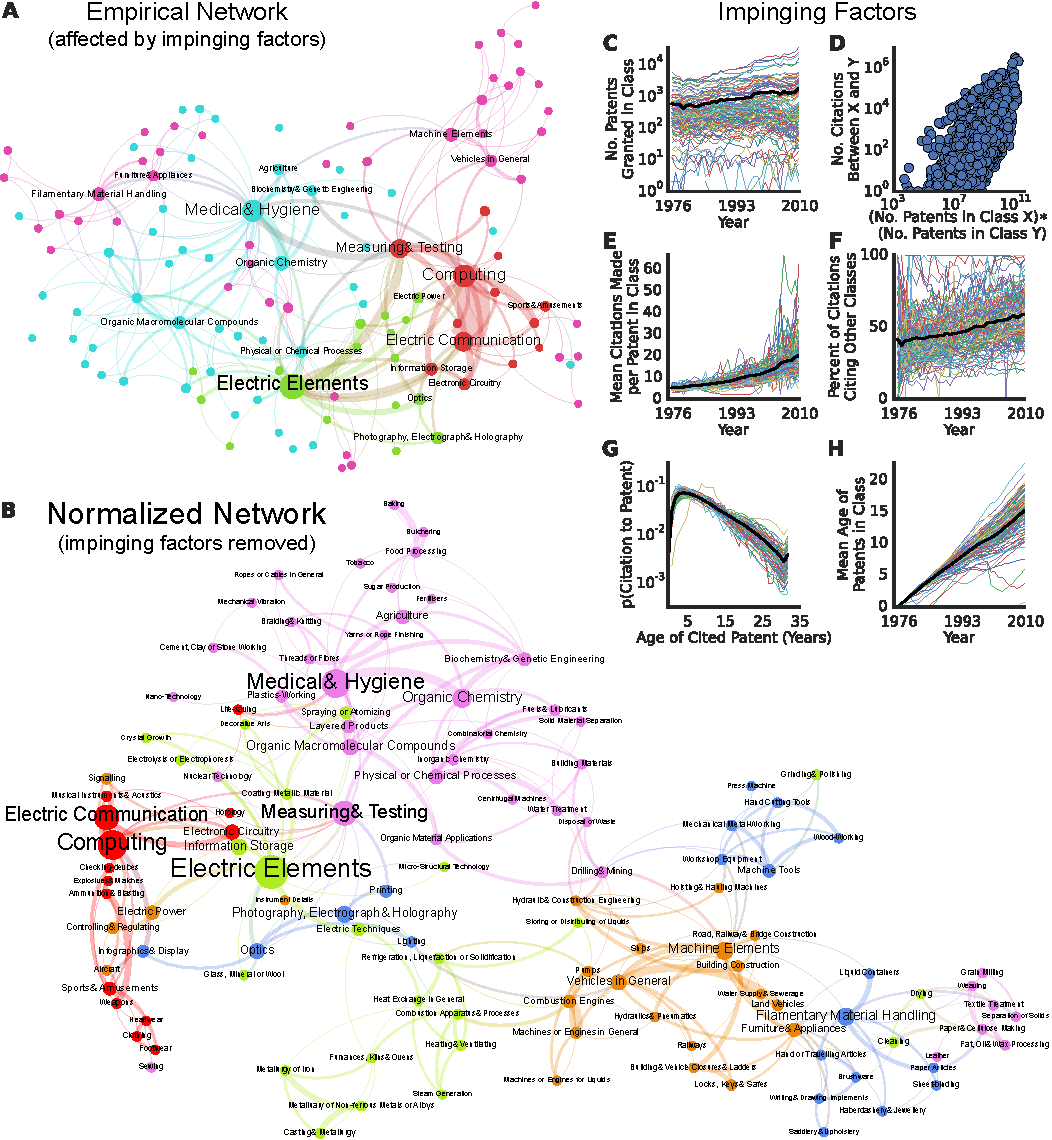
\includegraphics[]{figs/Network_and_Impinging_Factors.pdf} 
\end{center}
\caption{\textbf{Measuring technology relatedness networks that control for impinging factors reveals different network structures.} A-B) The empirical (A) and normalized (B) technology relatedness networks. Node size: the number of patents in the technology class. Link weight: proportional to the number of citations between the technology classes (the average of both directions). The networks are fully connected, but only a subset of the strongest links are visualized (see Materials and Methods). For visual reference, a community structure is shown by node color, which was identified using both visualized and unvisualized links. C-H) Aspects of the patenting system that affect citation rates, which thus impinge on measures of relatedness. The impinging factors vary greatly between technology classes and are not stable over time, but these complexities can be removed from measures of technology relatedness by normalizing with randomized controls. Colored lines: Individual classes. Black lines: Averages.
C) The number of patents in different technology classes, over time.
D) The number of citations between every pair of classes, which on average is proportional to the number of patents in the two classes.
E) The mean number of citations made by patents in different technology classes, over time. 
F) The percent of citations that cite patents in classes different from that of the citing patent, grouped by the class of the citing patent, over time.
G) The distribution of the ages of patents that are cited, grouped by the year the citation was made.
H) The average age of patents in different technology classes over time. The data for G and H are censored, as they only cover patents awarded from 1976 onward. 
}\label{Empirical_Normalized_Networks}
\end{figure*}

Here we show how to precisely control for the complexities of multiple impinging factors in patent data, all at once. We calculated a null hypothesis: an expectation of what the observed relatedness measure between two technology classes would be by random chance, given the other influencing factors. We then identified which pairs of technology classes had significantly higher relatedness than that expected by chance, revealing a sparse network. After normalizing the empirical relatedness measures relative to the random expectation, the different measures of technology relatedness became more correlated. The structures of the normalized technology network also coincided with human behavior: inventors' patenting histories closely followed the networks' structures. These results indicate that controlling for the impinging factors brings us closer to measuring the true technology space. 

\section{Factors Affecting Technology Relatedness Measures and How to Control for Them}

\subsection{Citations}
Patents cite other patents as related technologies, and the purpose of the citations is to limit what the citing patent can claim as intellectual property.Citations can thus represent knowledge proximity or knowledge use. We measured how often patents in two classes cited each other directly (Direct Citation
), how often classes were cited together by the same patents (Co-Citation
), how similar were the patterns of citations classes made or received from all other classes (Cosine Similarity, Inputs and Cosine Similarity, Outputs
) and how similar were the patterns of citations classes made or received from all other patents (Cosine Similarity, Inputs, High Resolution and Cosine Similarity, Outputs, High Resolution). These different measures have typically been used to capture different aspects of how technologies relate to each other (\textit{SI Text}). All of them, however, rely on patents' citations. Unfortunately, the probability of a citation between two patents, or between two technology classes, is affected by several variables that are not intrinsic properties of the inventions they represent \cite{Hall2001, Uzzi2013}. 

The expected number of citations between any two technology classes depends on several factors, which vary greatly across classes and time (Fig. \ref{Empirical_Normalized_Networks}C-H). First, the expected number of citations between a citing class and a cited class is driven by the number of patents in each (Fig. \ref{Empirical_Normalized_Networks}C,D). The number of citations is also affected by a class' propensity to make citations and in particular to cite patents in other classes (Fig. \ref{Empirical_Normalized_Networks}E,F). Lastly, patents are more likely to cite patents of a particular age, so the ages of patents in the cited class is also relevant (Fig. \ref{Empirical_Normalized_Networks}G,H). All of these phenomena are complex, but they are not properties of the technologies that patents represent; they are due to the patenting and inventive process (described in \textit{SI Text}). These factors thus impinge on the measures of relatedness that use citations, whose influence we can remove. 

To clean the empirical signal of technology relatedness from possible spurious relationships caused by the impinging factors, we compared the empirical relatedness values to a null hypothesis: What would the measured relatedness be by chance, given all the impinging factors? We calculated the random expectation by creating 1,000 randomized versions of the patent citation history, in which all of the impinging factors were exactly preserved. To create these randomized controls we identified groups of citations in which all the following properties were the same: the year the citing patents were issued, the year the cited patents were issued, and whether the citing and cited patents were in the same class (cross-class vs. same-class citations). For same-class citations, we only created citation groups in which all patents were in the same class. We then shuffled the cited patents among the citations in the group (Fig. \ref{citation_rewiring_diagram}). Perhaps surprisingly, virtually all citations were able to be grouped with other, similar citations and shuffled in this way (\textit{SI Text}). The resulting shuffled versions of the network were thus different from the original, but preserved all the desired features of the number of patents in each class, the patent age sequence, etc. 

\begin{figure}[]
\begin{center}
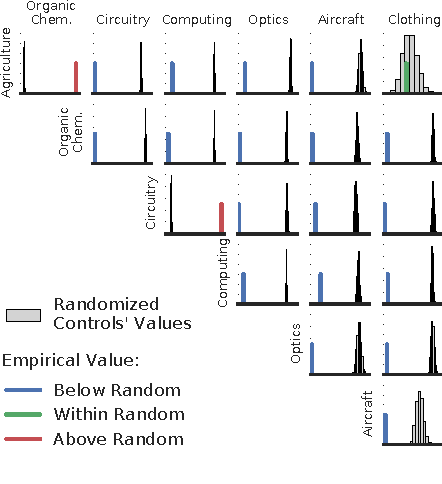
\includegraphics[width=\columnwidth]{figs/Rewiring_Histogram.pdf} 
\end{center}
\caption{\textbf{The empirical relatedness value of a link between any two classes was compared to the distribution of relatedness values across 1,000 randomized controls for that link.} Each panel represents the link between two classes, the row class (e.g. Agriculture) and the column class (e.g. Clothing). The relatedness metric shown is Co-Citation, the number of patents that cited patents in both the row class and the column class. Histogram: the distribution of relatedness values for that link across 1,000 randomized controls. Vertical lines: the empirical value for that link derived from the original patent citation network, colored by whether it is below, within, or above the values of the randomized controls. The empirical relatedness value for a given link was typically completely outside the distribution of the randomized controls' relatedness values for that link (see Fig. \ref{related_unrelated_percentages}). The panels shown are a small sample of the 7,260 possible links in the network.}\label{rewiring_histogram}
\end{figure}

We used the randomized patent citation history to calculate the different relatedness measures between the technology classes. For each pair of classes, we obtained a histogram of measured relatedness values across the 1,000 randomized controls (Fig. \ref{rewiring_histogram}, gray bars).\footnote{For certain measures and conditions it is possible to calculate the complete probability distribution for the randomized controls, using analytic approximations 
(\textit{SI Text}). The numeric solutions, however, are valid across all conditions and all measures.} We compared this histogram to the relatedness value calculated from the empirical patent citation history (Fig. \ref{rewiring_histogram}, vertical lines). For most pairs of classes the empirical relatedness measure was different from all 1,000 of the randomized control values, sitting entirely outside the histogram. This is analogous to the empirical link having a p-value below 0.001.

We summarized the difference between the empirical relatedness and the random expectation by computing the expected value and the standard deviation of the numerically-obtained distribution, then expressing the empirical relatedness measure as a z-score of the randomized controls. These z-score values were the normalized relatedness measure; this was the desired measure of ``true'' technology relatedness. 

Empirical and normalized link weights could convey very different perspectives.
For example, the empirical number of citations from ``Computing" to ``Electric Elements" seemed large at $56,349$, which put it in the top percentile of link weights. However, this was actually fewer citations than would be expected by chance: the randomized histories had $104,475 \pm 293$ citations between the two classes, and thus the normalized link weight was $-164$, in the bottom percentile of link weights.

\subsection{Co-Classification and Co-Occurrence}
Patents are assigned a main class to which they primarily belong, which is the class used for the citation analysis. But patents are also frequently assigned to additional, secondary classes. We can then measure how often two classes both appear on the same patents together (Co-Classification). Similarly, an inventor or firm can have multiple patents, and those patents could be in multiple classes. We can then measure how often two classes both appear together in inventors' and firms' patent histories (Co-Occurrence). Co-Classification is interpreted as measuring how often two technology domains are combined into an invention, while Co-Occurrence is interpreted as how often two technology domains are both used within a single mind or collection of minds (i.e. a firm). 

Like citations, Co-Classification and Co-Occurrence measures are also influenced by other impinging factors, such as the simple number of occurrences: A given technology class may be very common or very rare across all patents, inventors, or firms.
Similarly, each patent, inventor, or firm may associate with very many technology classes, or very few.
Controlling for the number of occurrences in co-occurrence data has been addressed in information science% \cite{Eck2009}
, ecology% \cite{Ulrich2007, Stone1990}
, medicine %\cite{Gobbi2014}
and economics %\cite{Neffke2008}
 \cite{Eck2009,Ulrich2007,Stone1990,Gobbi2014,Neffke2008}; it also markedly affects the observed relatedness of technology classes \cite{Bottazzi2010, Sanders2003}. We extend on this understanding by also controlling for temporal effects, since the number of occurrences of a class, patent or entity can vary over time. While some classes are popular in some years and not in others, a change in popularity ought not influence the true relatedness between technology classes. For example, if a firm only worked on what was most popular every year, the firm's activity would not provide new information on how technologies are related. Controlling for temporal effects allows us to measure how unusual it is that two classes co-occurred, given when they were each popular.

We controlled for the impinging factors in Co-Classification and Co-Occurrence measures by again comparing the empirical data to randomized controls. We created randomized versions of the patent record in which the number of associations made by each class, entity and patent was preserved. We also preserved temporal effects by treating each year of patent data separately, randomizing each individually, then combining them into a single, randomized version of history. We created 1,000 randomized controls in this way, described in more detail in \textit{SI Text}. We again compared the relatedness measures calculated from the randomized controls to those of the empirical values, as with the citations in Fig. \ref{rewiring_histogram}.

\section{Findings}


\subsection{The Technology Relatedness Network is Sparse}
Before normalizing relatedness measures, it is difficult to quantify the relatedness between two technologies and then assert if the resulting number is a high or low value.
However, comparing an empirical link weight to randomized controls yields a natural interpretation for whether a link is particularly strong or weak: an empirical link weight is stronger or weaker \textit{than would be expected by chance.} Most links in the relatedness networks were weaker than would be expected by chance (Fig. \ref{related_unrelated_percentages}), measured as being below the link weights of any of the 1,000 randomized controls (analogous to p<.001). For most relatedness measures, \textasciitilde{}20\% of the links were stronger than chance, indicating the two technology classes they connected were particularly related. 

The technology relatedness networks were thus sparsely connected, though sparse is a relative term; the network had 7,260 possible links, and with a link density 20\% there were still 1,452 links remaining. Still, controlling for spurious factors quantifies an intuitive fact: most technologies are not particularly related to each other. Instead, any single technology is only notably related to about 1 in 5 of the other technology domains.

Sparsity was notably not the case for the Co-Occurrence measured from firms' patenting histories: \textasciitilde{}50\% of technology pairs occurred together in firms' patenting histories at rates greater than chance. We also analyzed the patenting histories of countries and found a similar pattern, though the comparatively small sample of <200 countries meant the trend was not statistically significant (\textit{SI Text}).

\begin{figure}[]
\begin{center}
\includegraphics[]{figs/Related_Unrelated_Percentages.pdf} 
\end{center}
\caption{\textbf{Only \textasciitilde{}20\% of links between classes had a higher relatedness than that expected by chance.} Technology relatedness networks created using different metrics were compared to 1,000 randomized controls, by comparing the weights of their links. For most networks, a majority of the empirical links were below than any of the randomized controls (blue), and a minority were above the randomized controls (red). The exception were Co-Occurrence, Firm networks, which had \textasciitilde{}50\% of links above what would be expected by chance. 
}\label{related_unrelated_percentages}
\end{figure}


\begin{figure}[]
\begin{center}
\includegraphics[]{figs/Network_Correlations_Linear.pdf} 
\end{center}
\caption{\textbf{Normalizing networks made technology relatedness networks more similar to each other, while less influenced by other factors.}  Correlations are between the link weights of technology relatedness networks created with different measures of relatedness. Also included are the expected link weights if weight were proportional to a technology class' number of patents, which were uncorrelated with normalized relatedness networks. 
Lower left) Empirical networks.
Upper right) Normalized networks. Normalized networks' link weights are z-scores, where a link value of the empirical network is expressed as a z-score of the randomized controls' values for that link. Scatter plots of the raw data for all comparisons of relatedness measures are in Fig. \ref{Measure_Comparison_Scatter_Plots}.
}\label{measure_correlations}
\end{figure}

\subsection{After Normalization, Relatedness Measures Correlate with Each Other, but Not Impinging Factors}

Normalization changed how the different kinds of relatedness measures compared to each other. Among the empirical networks (before normalization) there were three groups of correlated networks (Fig. \ref{measure_correlations}, lower left panel). In the first group were Direct Citation and Co-Citation, in the second were the four varieties of Cosine Similarity, and last was Co\hyp{}Classification.
After normalization, all of the relatedness measures fell into a single correlated group (Fig. \ref{measure_correlations}, upper right panel). Thus, removing impinging factors led to more agreement among the different measures of relatedness.

Importantly, the measures of technology relatedness no longer reflected other, impinging factors, such as the number of patents in each technology class. We compared the technology relatedness networks to what would be expected if link weight were simply proportional to the number of patents in each class (similar to Fig. \ref{Empirical_Normalized_Networks}D). Before normalization, several measures of technology relatedness correlated with classes' patent counts (Fig. \ref{measure_correlations}, bottom row). After normalization, the linear correlations dropped to virtually zero for all technology relatedness networks (Fig. \ref{measure_correlations}, right column).

\subsection{Inventors' Behavior Follows Other Relatedness Measures Closely, While Firms' Portfolios Follow Less Closely}
Inventors' patenting histories closely followed the technology relatedness network structure identified by the normalized measures. Pairs of technology classes' normalized rates of Co-Occurrence in inventors' patent histories was strongly correlated with the other citation- and classification-based networks (Fig. \ref{Relatedness_Behavior_Correlation}, blue bars). The normalized technology networks, then, not only began to converge on a common description of technologies' relatedness to each other, but to a description that also mirrored inventors' behavior. The technology network maps may thus provide explanation for why a single mind that is able to invent in ``organic chemistry" is also likely able to invent in ``agriculture": these technology domains are intrinsically related.

Firms' patent portfolios, in contrast, followed the technology relatedness networks less closely. Pairs of technology classes' normalized rates of Co-Occurrence in firms' patent histories were also correlated with the other networks, but only weakly or moderately (Fig. \ref{Relatedness_Behavior_Correlation}, green bars). The association between technology relatedness and inventive behavior is similar for firms and inventors, but the variance is much larger for firms, reducing the strength of the association (Fig. \ref{Measure_Comparison_Scatter_Plots}). Firms, then, are like inventors in that they tend to invent in classes related to those that they already have experience in; notwithstanding, deviations from this general pattern are much more common and sizable for firms. Previous research has used co-occurrence data to investigate whether firms preferentially diversify into related classes \cite{Bottazzi2010, Breschi2003, Teece1994}. The present results show that firms' patent portfolios are indeed influenced by how related are different technology domains, but this is just one, modest influence. Firms' decisions to enter into a new technology domain are also determined by such factors as market demand, the availability of capital and risk diversification. Furthermore, firms are less constrained than individual inventors; they can hire additional staff or acquire new ventures that can bring in new knowledge unrelated to a firm's previous capabilities. As such, firms' inventive behavior only partially reflects the technology relatedness space. 

\begin{figure}[]
\begin{center}
\includegraphics[]{figs/Relatedness_Behavior_Correlation.pdf} 
\end{center}
\caption{\textbf{Inventors closely followed the technology network maps derived from the normalized relatedness measures, while firms followed the maps less closely.} The normalized counts of how often two technology classes co-occurred in inventors' patenting history correlated with other normalized measures of technology relatedness (blue bars). The normalized counts of how often two technology classes co-occurred in firms' patent portfolios correlated only modestly with the other measures of relatedness (green bars). %Error bars: 95\% confidence intervals.
}\label{Relatedness_Behavior_Correlation}
\end{figure}

\section{Discussion} 
Normalizing technology network maps by controlling for impinging factors uncovers previously obscured information, such as the sparsity of technology relatedness. Normalization also leads to convergence of many of the different measures of relatedness, as seen through their increased correlation. This suggests the existence of a unique, latent technology space, which the methods presented here allow us to measure more effectively. We have still not measured this space perfectly, but already the present data corresponds to human behavior: inventors are particularly likely to invent in sets of technology classes that are connected by the sparse links of relatedness. 

The normalized technology relatedness networks measured here can now serve as a map for technology development. Both individual inventors and firms can locate themselves and their knowledge on the map and observe what technology domains are nearby in the technology space. Nearby domains are likely better targets for new invention over more distant domains. Inventors are particularly justified in using the map to guide their future inventions, since inventors who successfully patent in multiple domains typically do so in closely related domains. Firms are less justified in restricting themselves to targeting technology developing in solely those domains that are closely related to their existing knowledge base; they may instead hire additional inventors with new knowledge to roam further afield. For both inventors and firms, it may be possible to use the map to plan a long-term research path: starting in the domain where one currently has knowledge, one can target a series of domains that are always closely related to each other, but ultimately result in patenting in a domain very unrelated from one's origin. Thus, the normalized technology relatedness map can be a significant strategic tool. 

Strategies of following the map (or not) are justified if an individual or firm wants to behave like those who successfully patent. It is possible, however, to have a higher bar: to be an inventor whose patents receive many citations, or to be a firm whose inventions yield high financial returns. It remains to be seen whether high-performing inventors or firms follow the technology space differently from others, be that more closely, less closely, or with a more complex strategy like targeting particularly dense or sparse regions of the network. 

Technology is a complex system, but we can gain understanding of that system by mapping out its components and their relations to each other. With the more accurate map presented here it is possible to study technology development with a new level of clarity, including both aspects of technologies themselves and how humans interact with those technologies. Improved understanding of technologies and invention may ultimately inform better technology development policies, leading to more successful technology creation and management.

%%%%%%
\section{Materials and Methods}
\label{materialsandmethods}
\subsection{Patent Data and Classes}
We used all 3,911,050 utility patents issued from 1976 to 2010 by the United States Patent and Trademark Office (USPTO).
All patents were classified under two systems: the International Patent Classification system (IPC; 121 classes) and the United States Classification system (USPC; 430 classes). The USPTO has recently joined other national other patent offices to exclusively use the new Cooperative Patent Classification system (CPC), which is based on the IPC. In order to ensure our findings are the most relevant for the future, we focus here on results from the IPC, which is more similar to the modern CPC system. We also repeated the analysis using the USPC classification, and found qualitatively similar results (\textit{SI Text}).

\subsection{Entity Tracking}
Inventor and firm identities were tracked across patents using name reconciliation data from \cite{Li2014}. This data identified 2,756,508 inventors and 247,913 firms. Firm identity reconciliation, performed by \cite{Li2014} and based on \cite{Hall2001}, focused on linking assignee names to firms traded in the United States stock market and harmonizing spell variations. It did not merge firms' subsidiaries, which can be distinct entities with different knowledge, capabilities, and operations. 
\subsection{Network Visualization}
We visualized the empirical and normalized technology relatedness networks %for each relatedness measure 
(Fig. \ref{Empirical_Normalized_Networks}A-B)% and \textit{SI Text})
. We highlighted a community structure for each network, which was calculated by approximately maximizing the weighted modularity using a faster version of the Louvain method \cite{Newman2004, Blondel2008, Traag2015}. Only a subgraph of the networks' links were visualized: the planar maximally filtered graphs \cite{Tumminello2005}. These graphs contained the set of links with the highest weights that were also topologically planar, such that they could be laid out flat on a plane without links crossing.

\acknowledgments{%
JA, GT and JL designed the study. BY collected the data and visualized the networks. JA and GT developed and performed the analysis. JA, GT and JL wrote the paper. We thank Ulf Bissbort, Bikramjit Das, Tommaso Demarie, Francois Lafond, and Chris Magee for helpful discussions. This work was supported by the SUTD-MIT International Design Centre (IDG31300112) and by the Singapore Ministry of Education Tier 2 Academic Research Grants (T2MOE1403).
}

% \endtwocolumns
% \vskip24pt
% \twocolumns
% \renewcommand*{\bibfont}{\footnotesize}
% \AtNextBibliography{\scriptsize}
% \printbibliography[heading=none]




% \renewcommand{\refname}{}

% \begingroup
%     \setlength{\bibsep}{-2pt}
%     {\footnotesize
%     \bibliography{Exported_Items.bib}{}
%     }
%     \bibliographystyle{pnas2011}
% \endgroup

\newpage
% \newrefsection

% \newgeometry{oneside}
\beginsupplement

\section*{Supporting Information}

\section{Relatedness Measures}\label{relatednessmeasures}
\subsection{Direct Citation}
The most straightforward way to describe the relatedness between two technology classes is to simply count the number of citations between them \cite{Leten2007}. The Direct Citation measure is the total number of citations from patents in a class $X$ to other patents in another class $Y$. Because citations disclose the relevant prior art, the direct citation count between classes can be interpreted as an overall measure of the importance of the cited class as a technical input for the citing one. 

\subsection{Co-Citation}
Patents can make many citations, including to patents from multiple classes. If two classes are often cited together they may function well together as a input. The Co-Citation between two classes $X$ and $Y$ is the number of patents that cited patents from both $X$ and $Y$. Co-citation has been used to measure the relatedness of scientific fields and journals \cite{Uzzi2013, Wallace2009}.


\subsection{Cosine Similarity}
A more sophisticated measure of relatedness is not whether two classes cite each other, but if they cite other classes in a similar pattern. We count how many citations patents in a class $X$ make to patents in every other class ($Y$, $Z$, and so on). This is summarized as a class-class citation vector, $c_X$. If the class-class citation vector is the same for two classes, they have the same citation behavior, and are taken to be related. If they have entirely different vectors, they have entirely different citation behaviors, and are taken to be unrelated. We calculate the similarity of the two class-class citation vectors by taking the cosine of the angle between them, $cos(c_X, c_Y)$. 

Cosine similarity is a long-used measure for evaluating the relatedness of technology domains in patent data. The cosine index was introduced by Jaffe \cite{Jaffe1986, Jaffe1989}, who measured relatedness between pairs of technological fields (proxied by IPC classes) by computing the cosine of the vectors representing the occurrences of fields in firms' patent documents. Breschi and colleagues \cite{Breschi2003}, designed a similar version of the index, which measures relatedness between class pairs as the cosine of the classes' vectors of co-occurrences in patent documents. 

Cosine similarity can be calculated using two different class-class citation vectors: the vector of citations the class $X$ \textit{makes} to every other class, and the vector of citations the class \textit{receives} from every other class. These can be thought of as measuring the similarity of knowledge inputs to the class vs. the similarity of knowledge outputs of the class. We refer to these two measures as Cosine Similarity, Inputs and Cosine Similarity, Outputs.

The principle of measuring class-class citation vectors can be extended to class-patent citation vectors. In this case, we measure how many citations patents in a class $X$ make to every individual patent, without summarizing them by which classes those patents are in. This creates a much higher dimensional vector (as there are many more patents than classes), but the principle is the same. Obviously, the citation vector measured at the class-patent citation level has a higher granularity than its class-class counterpart. This can be interpreted as a measure of similarity of specific, rather than generic, knowledge inputs or outputs between classes. The class-patent citation vectors between two classes can again be compared using cosine similarity. Again there are two versions of the measure, depending on whether we measure the citations a class makes versus the citations a class receives. We refer to these two measures as Cosine Similarity, Input , High Resolution and Cosine Similarity, Output, High Resolution. 

\section{Origins of Factors Impinging on Citation Counts}
The simplest factor influencing the number of citations between two technology classes is the number of patents in them. Technology classes vary greatly in size, and those sizes change over time (Fig. \ref{Empirical_Normalized_Networks}C). All else equal, larger classes both make and receive more citations, and thus there is a linear correlation between the sizes of two technology classes and the number of citations between them (Fig. \ref{Empirical_Normalized_Networks}D).

Another possible influence of examiner behavior changing over time is the number of citations made per patent. The number of citations made per patent varies across technology classes and history, and is increasing over time (Fig. \ref{Empirical_Normalized_Networks}E). This may be a cognitive bias due to the growing pool of potential prior art (more previous patents) and patent electronic databases, which makes searching for prior art easier and thus assessing novelty more stringent.   

Patents' citations are also biased to be made to patents within the same class. Citations are often made by patent examiners \cite{Criscuolo2008, Alcacer2006}, and the examiners leverage the classification system to make citations. They first classify the patent, then search for potentially related patents \cite{2014}, and so are more likely to find relevant previous patents to cite within the same class. The portion of citations made to patents in other classes varies greatly depending on the class of the citing patent, and is also growing over time (Fig. \ref{Empirical_Normalized_Networks}F); these differences can be due to differences in examiner behavior or office policy. 

Another factor affecting citations is time. Recent inventions need time to be recognized and older technologies gradually become unused, though can potentially remain indefinitely \cite{Hall2001,Valverde2007}. Since a patent's citations reflect what technologies are relevant prior art to the invention, these temporal effects are reflected in the citation record: Fig. \ref{Empirical_Normalized_Networks}G shows the distribution of the age of patents at the time they are cited. Obviously, because the patent data we studied only extends to 1976, the maximum possible patent age depends on the year in which the citing patents was awarded.
The increased likelihood of citing patents from a particular point in history interacts with the growing number of new patents and the increasing number of citations they make. It also crucially interacts with the fact that technology classes vary in age. The average age of patents in a technology class varies across classes, and is increasing over history (Fig. \ref{Empirical_Normalized_Networks}H). The trend is increasing partly by construction, as we have no data before 1976, but the large variance for recent years is likely a real phenomenon.

Given all these citation phenomena, the expected number of citations between any two technology classes depends on their propensity to cite and be cited by other classes, their number of patents, the age distribution of their patents and their propensity to make and received citations.

\section{Effectiveness of the patent citation network randomization}

\begin{figure}
\begin{center}
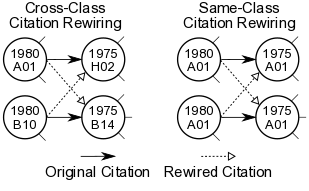
\includegraphics[width=\columnwidth]{figs/citation_rewiring_diagram_one_column.png} 
\end{center}
\caption{\textbf{The citation rewiring process used to create randomized control networks preserved many properties of the original patent citation network.} Citations were selected whose citing patents were issued in the same year and whose cited patents were also issued in the same year. Groups of citations were selected that were either all cross-class (left) or all same-class and all within the same class (right). The citations in the group were then shuffled. Performing this shuffling operation resulted in a randomized version of the patent citation network that still preserved many properties of the original networks, such as the cross-class citation rates, the time lag of citations, and the number of citations made and received by each patent. }\label{citation_rewiring_diagram}
\end{figure}

There are two wrinkles in how the generation of the randomized controls, which could in theory could affect the normalized relatedness measures, though in practice do not. The first wrinkle is that it is not guaranteed that for every citation there is another citation to be paired with that has all the same properties required. Fortunately, this happened rarely. Each citation was part of group of citations that had the same citing patent year, cited patent year, and cross-class identification (and for same-class citations, being within a particular technology class). Fig. \ref{rewiring_groups} shows the number of citations in each group that was represented in the patent network. Only approximately 14.16\% of citations were part of a group that fewer than 10 members. 2.55\% of citations were part of a group with 1 member; these were unique citations, and could not be rewired. Leaving these citations unaltered made the randomized control networks more similar to the empirical network. As discussed in the main text, the randomized control networks and the empirical network were still very different, and so the effect of the unrewired links was unappreciable.

\begin{figure}[h]
\centering
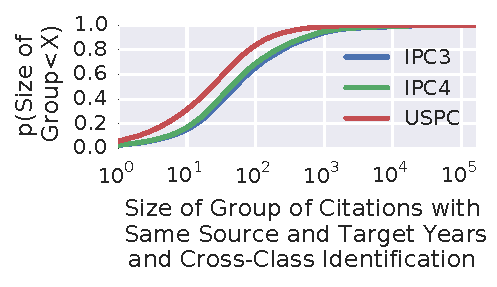
\includegraphics[]{figs/Citation_Group_Sizes.pdf} 

\caption{\textbf{Most citations had many other citations with the same properties, and so could be rewired.} The rewiring procedure used to create randomized controls required pairing each citation with another citation with similar properties (Fig. \ref{citation_rewiring_diagram}). If the group of citations with those properties was small, then that link would not have many opportunities for rewiring, and so the randomized controls would be similar to the empirical network. Over 85\% of citations were in a group that had 10 or more members. Only 2.55\% of citations were unique and could not be rewired. In practice, the empirical networks rarely resembled the randomized controls (Fig. \ref{related_unrelated_percentages})}\label{rewiring_groups}
\end{figure}

The second wrinkle of this normalization method is with rewiring cross-class citations. As in Fig. \ref{citation_rewiring_diagram}, if all four patents are from different classes, the desired outcome is achieved. However, it is possible that the citing patent of one citation is in the same class as the cited patent of the \textit{other} citation. In this case, both citations are indeed cross-class citations, but after rewiring one of the citations would become a same-class citation. Thus, the cross-class citation rate would decrease in the randomized controls, and the same-class citation rate would decrease (Note that it is not possible for the reverse mistake to occur, because all the same-class citations are paired and swapped separately.). The solution, of course, is to check that the paired citations do not have the problematic arrangement of classes, and so will not create a same-class citation. While this works in principle, it does not in practice. The solution requires checking, rejecting, and resuggesting possible pairs of citations. This process creates significant computational problems, and it is hard to assess if and when the process will even converge. Because of this, we left the problem in place, and so the randomized controls had an increased rate of same-class citations. This rate was small, with the rate of same-class citations raising from 39.74\% in the empirical patent citation network to a typical rate of 41.2\% in randomized controls. The decrease in cross-class citations in the randomized control patent citation networks would typically make the empirical network appear to have an unusually high amount of citations between two classes, leading to an unusually strong connection in the technology relatedness network. However, as discussed in the main text, the empirical network generally had much lower relatedness values than would be expected by chance. As such, the error that the imperfect rewiring introduces would only make the unusually low normalized values more notable.

\section{Randomization of Co-Classification and Co-Occurrence Data}
 The process for controlling for the number of occurrences of each class and the number of associations of each patent or entity is the same principle as used in the patent citation network: many randomized control versions of the empirical data are created.  In the randomized controls, the number of occurrences of each class and the number of associations of each patent or entity is preserved, but the assigning of technology classes to patents or entities is otherwise random. This goal is practically accomplished by expressing the co-classification or co-occurrence data as a bipartite graph, in which technology classes are one type of node and they form connections to another type of node, be that patents or entities. Randomized controls are then created by shuffling the bipartite network's links, but preserving each node's degree. The bipartite network is then projected into a single-mode network, the co-classification or co-occurrence network. The resulting one-mode network is then compared to the same information from the empirical, unrandomized data.

The bipartite network is  equivalent to a binary matrix, with patents or entities forming the rows and technology classes forming the columns. Reshuffling the bipartite network is equivalent to creating random versions of the binary matrix, with each row and column having the same sum. Bottazzi and Pirino described how creating random controls in this way for co-occurrence data can markedly alter the interpretation of empirical co-occurrences \cite{Bottazzi2010}. We extend the shuffling technique they used with a reshuffling method designed with bipartite networks in mind \cite{Gobbi2014}. These methods analytically determine the number of rewires necessary to make on the original bipartite network in order to effectively take an unbiased sample from the set of networks with the same degree sequence. We used the BiRewire software package to first calculate the necessary number of rewires for each of the bipartite networks we examined, and then to rapidly execute the rewires \cite{Gobbi2015}.

We created randomized controls that preserved temporal changes in class' popularity and entity's activity by treating each year of data as a separate bipartite network. Each year was rewired independently, and then all years were combined to create the final randomized control to which the empirical network was compared.

Preserving temporal behavior introduces information which is not typically considered in the analysis of co-occurrence data. It also introduces additional complexity. Consider an inventor who was active in one technology class: \textit{Hats}. This inventor was active for 10 years, patenting each year, each time in the technology class for \textit{Hats}. If we identify this inventor as "occurring" in \textit{Hats} each year, and randomize each of the 10 years individually, it is likely that across the 10 randomized years the inventor will then occur in  many different technology classes. When we combine the 10 randomized years back together, we would then observe that the inventor occurred in many technology classes, perhaps 10, which is far more than the 1 class in which the inventor was actually active. By marking the inventor as "occurring" in every year individually, our randomization will thus break the  basic task of preserving the number of classes the inventor was active in. Therefore, any time an inventor or firm is awarded patents in a class in multiple years, we have a problem.

The solution to the problem of an entity "occurring" over multiple years is to not consider the entity as occurring over multiple years. Instead, the entity is considered to occur in each class only once, in a single year. In this way, randomizing each year individually cannot increase the total number of classes that an entity associates with in its history. After randomization of individual years and combining them together, the number of classes per entity and entities per class will still be preserved. 

For the purpose of entities patenting in technology classes, the most salient year to mark the entity as occurring in a class is the \textit{first} year that entity patented in that class. This is particularly relevant for controlling for phenomena like popularity-chasing; if a firm only enters technology domains because they are popular, that does not provide more information about how related technology domains are. We thus mark each entity as occurring in a technology class when they first entered into that class, and compare to randomized controls that preserve the timing of the entries.

\subsection{Preserving Temporal Information Markedly Affected Firm Measures, but not Others}
Preserving the year sequence in the randomized controls had only a modest effect on the measured normalized network, for most measures (Fig. \ref{CoOccurrence_Year_Preservation_Comparison}). However, the Co-Occurrence, Firm measure was markedly altered by preserving the year sequences. Without preserving year sequences, the Co-Occurrence, Firm network had \textasciitilde{}25\% of its links stronger than random chance, closer to the fraction observed in the other relatedness measures. By preserving the year sequences in the randomized controls and normalizing out such phenomena as popularity-chasing, the normalized Firm, Co-Occurrence network had \textasciitilde{}50\% of links stronger than chance.

\begin{figure}[]
\centering
\includegraphics[width=.5\textwidth]{figs/CoOccurrence_Year_Preservation_Comparison.pdf} 
\caption{\textbf{Most relatedness measures were only modestly affected by preserving yearly history.} The exception was in Co-Occurrence, Firm, which showed a marked change in the number of links that were stronger than chance.}\label{CoOccurrence_Year_Preservation_Comparison}
\end{figure}

By preserving temporal effects, the Co-Occurrence of technology classes in firms' patent portfolios were found to be generally more frequent than chance. Thus, by creating randomized controls that had more features in \textit{common} with the empirical data (the temporal sequence), the empirical data appeared more \textit{unusual}. This may seem counter intuitive, and so we provide some intuition here. Consider two statements:
\begin{quote}
1. "I am a human, and I speak Mandarin Chinese". 
\end{quote}
This is unusual, but not that unusual. A randomly selected human has about a 1/7 chance of speaking Mandarin Chinese.

\begin{quote}
2. "I am an Italian human, and I speak Mandarin Chinese".
\end{quote}
This is very unusual. A randomly selected Italian human has a much lower chance of speaking Mandarin Chinese.

Thus, by adding additional constraints to the randomized controls, we generate controls that are more like the empirical sample (human vs. Italian human), but the empirical sample is now more different from the controls.

In our case, we generate randomized controls that can either:
\begin{enumerate}
\item freely associate classes with firms, regardless of firms' histories
\item must associate classes with firms only when the firms entered a new class
\end{enumerate}

Consider a class, \textit{Hats}, that had some level of popularity $P$ across all of history, but during some periods of history had a much smaller popularity, $p$. Using method 1, randomized controls will match up a firm with \textit{Hats} at the rate $P$. However, it is possible that a specific firm only entered a new class at the moment in history when \textit{Hats} had the diminished popularity $p$.  Method 1 is blind to this fact. However, using method 2, randomized controls will match up the firm with \textit{Hats} at the rate $p$. The specific firm's entry into \textit{Hats}, then, appears more unusual using method 2 than method 1, because $p<P$. 

Therefore, using randomized controls that preserve the yearly sequence of firms' entries can identify temporal effects that make a firm's movement into a class appear more unusual. This method can then be scaled to a whole population of firms, to determine if their movements in aggregate are unusual. We can then measure whether the co-occurrence of two classes in firms' portfolios is unusual, i.e. different from that expected by chance.

\begin{figure*}[]
\centering
\includegraphics[]{figs/Measure_Comparison_Scatter_Plots.png} 
\caption{\textbf{Comparison of link weights across different relatedness measures.} Blue: empirical networks. Red: normalized networks. Black. empirical vs. normalized for each measure compared to itself (x-axis: empirical, y-axis: normalized). 
}\label{Measure_Comparison_Scatter_Plots}
\end{figure*}



\section{Co-Occurrence, Country Data}
The empirical relatedness links between technology classes had values typically much higher or lower than all 1,000 randomized controls, across all measures of relatedness (Fig. \ref{related_unrelated_percentages}). We measure this phenomena in more detail by expressing each empirical link's value as a percentile rank, relative to the randomized controls. Fig. \ref{p_value_histograms} shows the histograms of the empirical links' ranks, for each relatedness measure. For the nine relatedness measures reported in the main text, the majority of links were lower than all randomized controls (rank 0) or higher (rank 100). For eight of the relatedness measures, rank 0 links outnumbered rank 100 links. The exception was the Co-Occurrence, Firm network, in which rank 100 links were more common than rank 0 links.

We analyzed the patenting histories of countries to create a Co-Occurrence, Countries network, analogous to the networks created from Co-Occurrence, Inventor and Co-Occurrence, Firm measures. The country data was similar to the firm data, in that rank 100 links were more common than rank 0 data (Fig. \ref{p_value_histograms}, lower right panel). However, the vast majority of links between technology domains were between ranks 0 and 100, meaning they had values within the range expected by chance (covered by the 1,000 randomized controls). It is possible that with additional country data these links would prove to be significantly different from chance. However, with less than 200 countries, the co-occurrence data did not provide a sufficiently strong signal to assert that country's invention portfolios combined many technology classes at rates different from random chance.

\begin{figure}[h]
\centering
\includegraphics[width=.5\textwidth]{figs/Country_CoOccurence_Histograms.pdf} 
\caption{\textbf{All relatedness measures found that most technology relatedness links were very different from randomized controls, except Co-Occurrence, Country.}}\label{p_value_histograms}
\end{figure}

\section{Analytic Approximations of Randomized Controls}
\subsection{Expected Number of Citations}
The expected value of citations between any pair of classes and its standard deviation can be conveniently approximated analytically by exploiting the statistical properties of our randomization process. The process can be seen as a sum of random variables $X_{t,lag}$, one for each citing-cited year ${t,lag}$ pair that describe the possible relationship between a given citing and cited class. The citation swapping procedure can be described as sampling a number of citations $n_{citing_{t,lag}}$ without replacement out of a population $N$ of \textit{swappable} citations that respect the required constraints, in which there are exactly $K$ citations directed toward the given cited class. Therefore, for each citing-cited year pair ${t,lag}$, the expected number of citations between a citing and a cited class behaves like a hypergeometric random variable $X_{t,lag}$. As such, the total expected number of citations for a given pair of citing-cited classes is described by the sum ${C_{citing,cited}}$ of hypergeometric random variables ${X_{t,lag}}$ with different number of trials \textit{n}, population size $N_{t,lag}$ and number of successes $K_{cited_{t,lag}}$. It follows that the expected value $E(C_{citing,cited})$ is approximately equal to

\begin{multline}
E(C_{citing,cited}) \sim \sum_{\forall t \in T_{citing}}\sum_{lag=0}^{t-1976} \bigl[ n_{citing_{t,lag}} \\
* p(connection)_{cited_{t,lag}} \bigr]
\end{multline}\label{expected_value_citation}

Where $n_{citing_{t,lag}}$ is the number of citations made by the given citing class to be reshuffled for each random variable $X_{t,lag}$ (i.e. the number of trials). The probability of swapping any of these citations with anyone connecting to a patent belonging to the given cited class is

\begin{equation}
p(connection)_{cited_{t,lag}} = \frac{K_{cited_{t,lag}}}{N_{t,lag}}
\end{equation}\label{probability_connection}

More specifically, for each citing-cited year pair ${t,lag}$ the number of trials $n_{citing_{t,lag}}$ is equal to

\begin{equation}
n_{citing_{t,lag}} = C_{citing_{t}} p(lag)_{citing_{t,lag}} p(outward)_{citing_{t,lag}}
\end{equation}\label{number_of_trials}

Where $C_{citing_{t}}$ is the number of citations made by patents granted in year \textit{t} belonging to the given citing class, $p(lag)_{citing_{t,lag}}$ is the probability that they cite patents granted in the year ${t-lag}$ and $p(outward)_{citing_{t,lag}}$ is the probability that they cite patents belonging to a class different from the one of origin. The latter two are indexed by $citing$, $t$ and $lag$ because, as we have shown in the panels of Fig. \ref{Empirical_Normalized_Networks}, there is a large variability across classes and time. It follows that the standard deviation $\sigma_{citing,cited}$ of ${C_{citing,cited}}$ is approximately equal to

\begin{multline}\label{standard_deviation}
\sigma_{citing,cited} \sim 
\sqrt{ 
\sum_{\forall t \in T_{citing}}\sum_{lag=0}^{t-1976} \bigl[ n_{citing_{t,lag}}} \\
\shoveright{* p(connection)_{cited_{t,lag}}} \\
\shoveright{* (1-p(connection)_{cited_{t,lag}})} \\
* \frac{N_{t,lag}-n_{citing_{t,lag}}}{N_{t,lag}-1} \bigr]  
% } 
\end{multline}

When $N_{t,lag}$ is large and $n_{t,lag}$ is small compared to it, then the fraction in equation \ref{standard_deviation} approaches unity. Therefore, the $\sigma_{citing,cited}$ can be approximated by the standard deviation of a binomial distribution. This is particularly handy if one would like to have an analytic solution for the p-values of the empirical relatedness. In fact, the distribution of the sum of hypergeometric random variables with varying number of trials and probability of success has no closed form solution. However, the sum of binomial random variables with different $n$ and $p$, can be seen as the the sum of Bernoulli random variables with different probabilities and is, therefore, described by the Poisson binomial distribution (a.k.a. Bernoulli-Poisson distribution) \cite{Hong2013, Fernandez2010, Chen1997}. Recently, it has been shown that the Poisson-binomial cumulative and probability distribution functions have exact closed-form solutions and accurate refined normal approximations \cite{Hong2013}. Based on the equations discussed here it is straightforward to derive the expected value of co-citations and cosine similarity between classes by using the joint probability distribution of citations from patents to classes and the cosine value of the vectors of expected received citations for any given class pairs.
 
\subsection{Nature and Quality of the Analytic Approximation}
The solutions for $E(C_{citing,cited})$ and $\sigma_{citing,cited}$ reported above are excellent approximations of numeric solutions  for the number of citations between classes, as provided by our randomization process (Fig. \ref{Comparison_ANAvsNUM}). The same approach could be applied to predict the numeric solution of the expected value and variance of co-occurrences of classes in patents, inventors' and firms' patenting histories. In this case $n$ would be the number of classes in which a patent, an inventor or a firm have been inventing, $K$ would be the number of patents, inventors or firms that have been patenting in a given class and $N$ would be the total number of occurrences (i.e. of links) in a bipartite network of patents*classes, inventors*classes or firms*classes. However, the approximation would perform very poorly in this case. 

The source of the analytical approximation deviating from the real behavior is due to the binary nature of citation networks and bipartite occurrence networks. When one works with weighted networks, numeric solutions provided by randomization algorithms that preserve row and column sums of the adjacency matrix, and analytic solutions based on hypergeometric distributions fully agree. In contrast, with binary networks, analytic solutions based on hypergeometric random variables may considerably differ from numeric solutions. The source of the problem lays in the possibility of double counting associations. Suppose that we are measuring the expected number of citations between patents. Suppose also that patent $A$ cites patents $B$ and $C$ and that patent $D$ cites patents $B$ and $E$, and that we want to swap citations between patents. If we use a permutation algorithm (which are a popular choice for randomizing weighted networks) to randomize citations, we might incur in double counting. In our example, if we permute cited patents we might end up in a configuration in which patent $A$ cites patent $B$ twice and patent $D$ cites patents $C$ and $E$. This would obviously break the binary nature of patent citations networks, and make the model deviate from reality. If our example would now describe a fictitious weighted networks we would not be facing double-counting problems as the random realization of the network would just strengthen the link between node $A$ and node $B$. Algorithms like BiRewire randomize networks while automatically preserving row and column sums of the empirical adjacency matrix, but also avoiding the possibility of double counting associations (this is accomplished by repeatedly swapping associations within sub-matrices of four cells in which associations are only found in one of the two diagonals). Analytic approaches based on hypergeometric distributions provide the exact solutions for permutation algorithms and are blind to the possibility of double-counting. Therefore, if we use them to predict expected values and standard deviation of associations between nodes in binary networks, we incur a mistake.

When we deal with a large patent citation network, in which the in-degree distribution is extremely skewed (i.e. most of the nodes have a very low $K$), most of the patents cite several patents (i.e. $n$ is relatively large), and there are many links (i.e. $N$ is very large), the probability of selecting two citations to swap that will cause double-counting is very low. To understand this, suppose now that patent $A$ cites patents $B$ and $C$ (and therefore has $n=2$), that patent $B$ has been cited $K$ times and that there are $N$ citations in the network. We would face double counting of citations from patent $A$ to $B$ only if, during the randomization process, we would randomly pick the citations from $A$ to $C$ and swap it with another one directed to $B$. This will happen with probability $(1/n)*(K-1)/(N-n)$, which is very small. For these reasons, the hypergeometric-based analytic solution, designed to predict permutation algorithms, works very well in our case, even if we randomize our binary citation network by using a 2-by-2 sub-matrix diagonal swapping algorithm (Fig. \ref{Comparison_ANAvsNUM}), top row). However, for co-occurrence data, the situation is very different. 

The occurrence networks of patents-classes, inventors-classes and firms-classes have much fewer links than a patent citation network (i.e. $N$ is much smaller) and the occurrence of some classes is much more common that the appearance of citations to a given patent (i.e. $K$ is much larger compared to $N$ in our occurrence networks). Therefore, the probability of incurring in double counting, if we would use permutation algorithms, is much larger. Accordingly, 2-by-2 sub-matrix diagonal swapping algorithms, like BiRewire, must be used in this case and the misuse of hypergeometric-based analytic solutions to predict their outcome actually causes type I and II errors in the inference based on z-scores (Fig. \ref{Comparison_ANAvsNUM}, right column). For this reason, precise analytic solutions of the expected value and variance of occurrences of classes in patents, inventors' and firms' histories do not exist. We must therefore solely rely on the numeric solutions provided by our randomization method, to calculate reliable z-scores of technology relatedness.        
\begin{figure*}[]
\centering
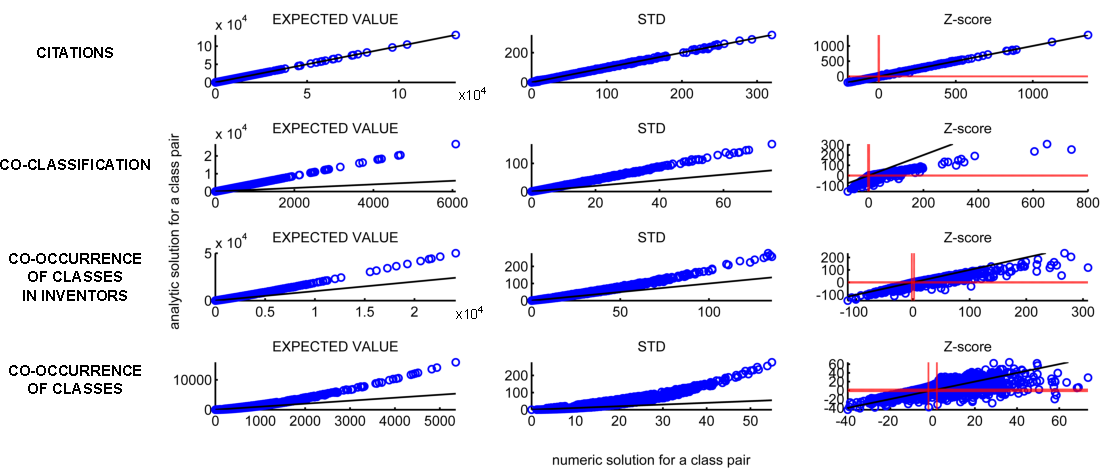
\includegraphics[width=\textwidth]{figs/Comparison_ANAvsNUM.pdf} 
\caption{\textbf{Comparison of analytic and numeric solutions of the expected value (first column), standard deviation (second column) and z-scores (third column) of direct citations (first row), co-classification (second row), co-occurrences of classes in inventors' patenting histories (third row) and in firms histories (fourth row).} One data point per class pair. If the analytic and numeric solutions would agree, all data points would lay on the black solid lines. This only happens for direct citations. Red shaded lines in the z-scores panel highlights values of the z-scores equal to 2 and -2, i.e. a possible threshold of statistical significance for relatedness and unrelatedness based on a normal approximation. Inference based on the analytic solutions would cause both type I and II errors for co-classification and co-occurrences. 
}\label{Comparison_ANAvsNUM}
\end{figure*}

\printbibliography
% \section{Analysis with USPC Classification System}
% \clearpage

\begin{figure}[p!]
\centering
\includegraphics[width=\columnwidth]{figs/USPC_figs/USPC_Impinging_Factors.png} 
\caption{\textbf{The impinging factors affecting relatedness measures, calculated using the USPC classification system.}}
\end{figure}

\begin{figure}[p!]
\centering
\includegraphics[width=\columnwidth]{figs/USPC_figs/USPC_Related_Unrelated_Percentages.pdf} 
\caption{\textbf{Using the USPC classification system, all measures of technology relatedness showed a sparse network after normalization.} About 10\% of links between technology classes were stronger than would be expected by chance, given the impinging factors. This is half the link density observed when using the IPC classification, which is to be expected from a higher resolution classification system. Like with the IPC analysis, the Co-Occurrence of patents in firms' patent histories had about twice the density of the other measures.}
\end{figure}

\begin{figure}[p!]
\centering
\includegraphics[width=\columnwidth]{figs/USPC_figs/USPC_Network_Correlations_Linear.pdf} 
\caption{\textbf{The different measures of technology relatedness, as calculated using the USPC classification system, had heterogeneous correlations before normalization. After normalization, however, all measures were strongly correlated.} Before normalization several measures between pairs of classes had some correlation with the number of patents in the two classes, but after this correlation was removed.}
\end{figure}

\begin{figure}[p!]
\centering
\includegraphics[width=\columnwidth]{figs/USPC_figs/USPC_Relatedness_Behavior_Correlation.pdf} 
\caption{\textbf{As calculated using the USPC classification system, the normalized measures of technology relatedness strongly correlated with the behavior of inventors, and modestly with the behavior of firms.}}
\end{figure}


% \section{Technology Relatedness Network Visualizations}

% \renewcommand{\dblfloatpagefraction}{0.1}
% \clearpage

% \begin{figure*}[p!]
% \centering
% \includegraphics[width=\textwidth]{figs/Network_Visualizations/Co_citation_empirical.pdf} 
% \caption{Visualization of the technology relatedness network created from the empirical Co-Citation measure.}
% \end{figure*}

% \begin{figure*}[p!]
% \centering
% \includegraphics[width=\textwidth]{figs/Network_Visualizations/Co_citation_zscore.pdf} 
% \caption{Visualization of the technology relatedness network created from the normalized Co-Citation measure.}
% \end{figure*}

% \begin{figure*}[p!]
% \centering
% \includegraphics[width=\textwidth]{figs/Network_Visualizations/Cosine_inputs_empirical.pdf} 
% \caption{Visualization of the technology relatedness network created from the empirical Cosine Similarity, Inputs measure.}
% \end{figure*}

% \begin{figure*}[p!]
% \centering
% \includegraphics[width=\textwidth]{figs/Network_Visualizations/Cosine_inputs_zscore.pdf} 
% \caption{Visualization of the technology relatedness network created from the normalized Cosine Similarity, Inputs measure.}
% \end{figure*}

% \begin{figure*}[p!]
% \centering
% \includegraphics[width=\textwidth]{figs/Network_Visualizations/Cosine_outputs_empirical.pdf} 
% \caption{Visualization of the technology relatedness network created from the empirical Cosine Similarity, Outputs measure.}
% \end{figure*}

% \begin{figure*}[p!]
% \centering
% \includegraphics[width=\textwidth]{figs/Network_Visualizations/Cosine_outputs_zscore.pdf} 
% \caption{Visualization of the technology relatedness network created from the normalized Cosine Similarity, Outputs measure.}
% \end{figure*}

% \begin{figure*}[p!]
% \centering
% \includegraphics[width=\textwidth]{figs/Network_Visualizations/Co_classification_empirical.pdf} 
% \caption{Visualization of the technology relatedness network created from the empirical Co-Classification measure.}
% \end{figure*}

% \begin{figure*}[p!]
% \centering
% \includegraphics[width=\textwidth]{figs/Network_Visualizations/Co_classification_zscore.pdf} 
% \caption{Visualization of the technology relatedness network created from the normalized Co-Classification measure.}
% \end{figure*}


% \begin{figure*}[p!]
% \centering
% \includegraphics[width=\textwidth]{figs/Network_Visualizations/Co_occurrence_inventor_empirical.pdf}
% \caption{Visualization of the technology relatedness network created from the empirical  measure of Co-Occurrence Counts in Inventors' Patents.}
% \end{figure*}

% \begin{figure*}[p!]
% \centering
% \includegraphics[width=\textwidth]{figs/Network_Visualizations/Co_occurrence_inventor_zscore.pdf} 
% \caption{Visualization of the technology relatedness network created from the normalized measure of Co-Occurrence Counts in Inventors' Patents}
% \end{figure*}

% \begin{figure*}[p!]
% \centering
% \includegraphics[width=\textwidth]{figs/Network_Visualizations/Co_occurrence_firm_empirical.pdf}
% \caption{Visualization of the technology relatedness network created from the empirical  measure of Co-Occurrence Counts in Firms' Patents.}
% \end{figure*}

% \begin{figure*}[p!]
% \centering
% \includegraphics[width=\textwidth]{figs/Network_Visualizations/Co_occurrence_firm_zscore.pdf} 
% \caption{Visualization of the technology relatedness network created from the normalized measure of Co-Occurrence Counts in Firms' Patents}
% \end{figure*}

% \begin{figure*}[p!]
% \centering
% \includegraphics[width=\textwidth]{figs/Network_Visualizations/Co_occurrence_country_empirical.pdf}
% \caption{Visualization of the technology relatedness network created from the empirical  measure of Co-Occurrence Counts in Countries' Patents.}
% \end{figure*}

% \begin{figure*}[p!]
% \centering
% \includegraphics[width=\textwidth]{figs/Network_Visualizations/Co_occurrence_country_zscore.pdf} 
% \caption{Visualization of the technology relatedness network created from the normalized measure of Co-Occurrence Counts in Countries' Patents}
% \end{figure*}


\end{document}
